\documentclass[12pt]{amsart}


\usepackage{times}
\usepackage[margin=1 in]{geometry}
\usepackage{paralist,amsmath,amssymb,multicol,graphicx,framed,ifthen,color,xcolor,stmaryrd,enumitem,colonequals}
\usepackage[outline]{contour}
\contourlength{.4pt}
\contournumber{10}
\newcommand{\Bold}[1]{\contour{black}{#1}}

\definecolor{chianti}{rgb}{0.6,0,0}
\definecolor{meretale}{rgb}{0,0,.6}
\definecolor{leaf}{rgb}{0,.35,0}
\newcommand{\Q}{\mathbb{Q}}
\newcommand{\N}{\mathbb{N}}
\newcommand{\Z}{\mathbb{Z}}
\newcommand{\R}{\mathbb{R}}
\newcommand{\C}{\mathbb{C}}
\newcommand{\e}{\varepsilon}
\newcommand{\inv}{^{-1}}
\newcommand{\dabs}[1]{\left| #1 \right|}
\newcommand{\ds}{\displaystyle}
\newcommand{\solution}[1]{\ifthenelse {\equal{\displaysol}{1}} {\begin{framed}{\color{meretale}\noindent #1}\end{framed}} { \ }}
\newcommand{\solutione}[1]{\ifthenelse {\equal{\displaysol}{1}} {\begin{framed}{\color{leaf}This solution is embargoed.}\end{framed}} { \ }}
\newcommand{\showsol}[1]{\def\displaysol{#1}}
\newcommand{\nosolfill}{\ifthenelse {\equal{\displaysol}{1}} {} {\vfill}}
\newcommand{\nosolpage}{\ifthenelse {\equal{\displaysol}{1}} {} {\newpage}}
\newcommand{\nosolonly}[1]{\ifthenelse {\equal{\displaysol}{1}} {} {{#1}}}

\newcommand{\rsa}{\rightsquigarrow}


\newcommand\itemA{\stepcounter{enumi}\item[{\Bold{(\theenumi)}}]}
\newcommand\itemB{\stepcounter{enumi}\item[(\theenumi)]}
\newcommand\itemC{\stepcounter{enumi}\item[{\it{(\theenumi)}}]}
\newcommand\itema{\stepcounter{enumii}\item[{\Bold{(\theenumii)}}]}
\newcommand\itemb{\stepcounter{enumii}\item[(\theenumii)]}
\newcommand\itemc{\stepcounter{enumii}\item[{\it{(\theenumii)}}]}
\newcommand\itemai{\stepcounter{enumiii}\item[{\Bold{(\theenumiii)}}]}
\newcommand\itembi{\stepcounter{enumiii}\item[(\theenumiii)]}
\newcommand\itemci{\stepcounter{enumiii}\item[{\it{(\theenumiii)}}]}
\newcommand\ceq{\colonequals}


\DeclareMathOperator{\ord}{ord}

\DeclareMathOperator{\res}{res}
\setlength\parindent{0pt}
%\usepackage{times}

%\addtolength{\textwidth}{100pt}
%\addtolength{\evensidemargin}{-45pt}
%\addtolength{\oddsidemargin}{-60pt}

\pagestyle{empty}
%\begin{document}\begin{itemize}

%\thispagestyle{empty}




\begin{document}
\showsol{0}
	
	\thispagestyle{empty}
	
	\section*{Calculator numbers}
	\begin{framed}
\textsc{Definition:} A \textbf{dollar store calculator} is a device that allows you to enter numbers with finite decimal expansion, and apply the operations $+,-,\times,\div$ and $\surd$.	
A dollar store calculator can only work with real numbers.

\begin{center}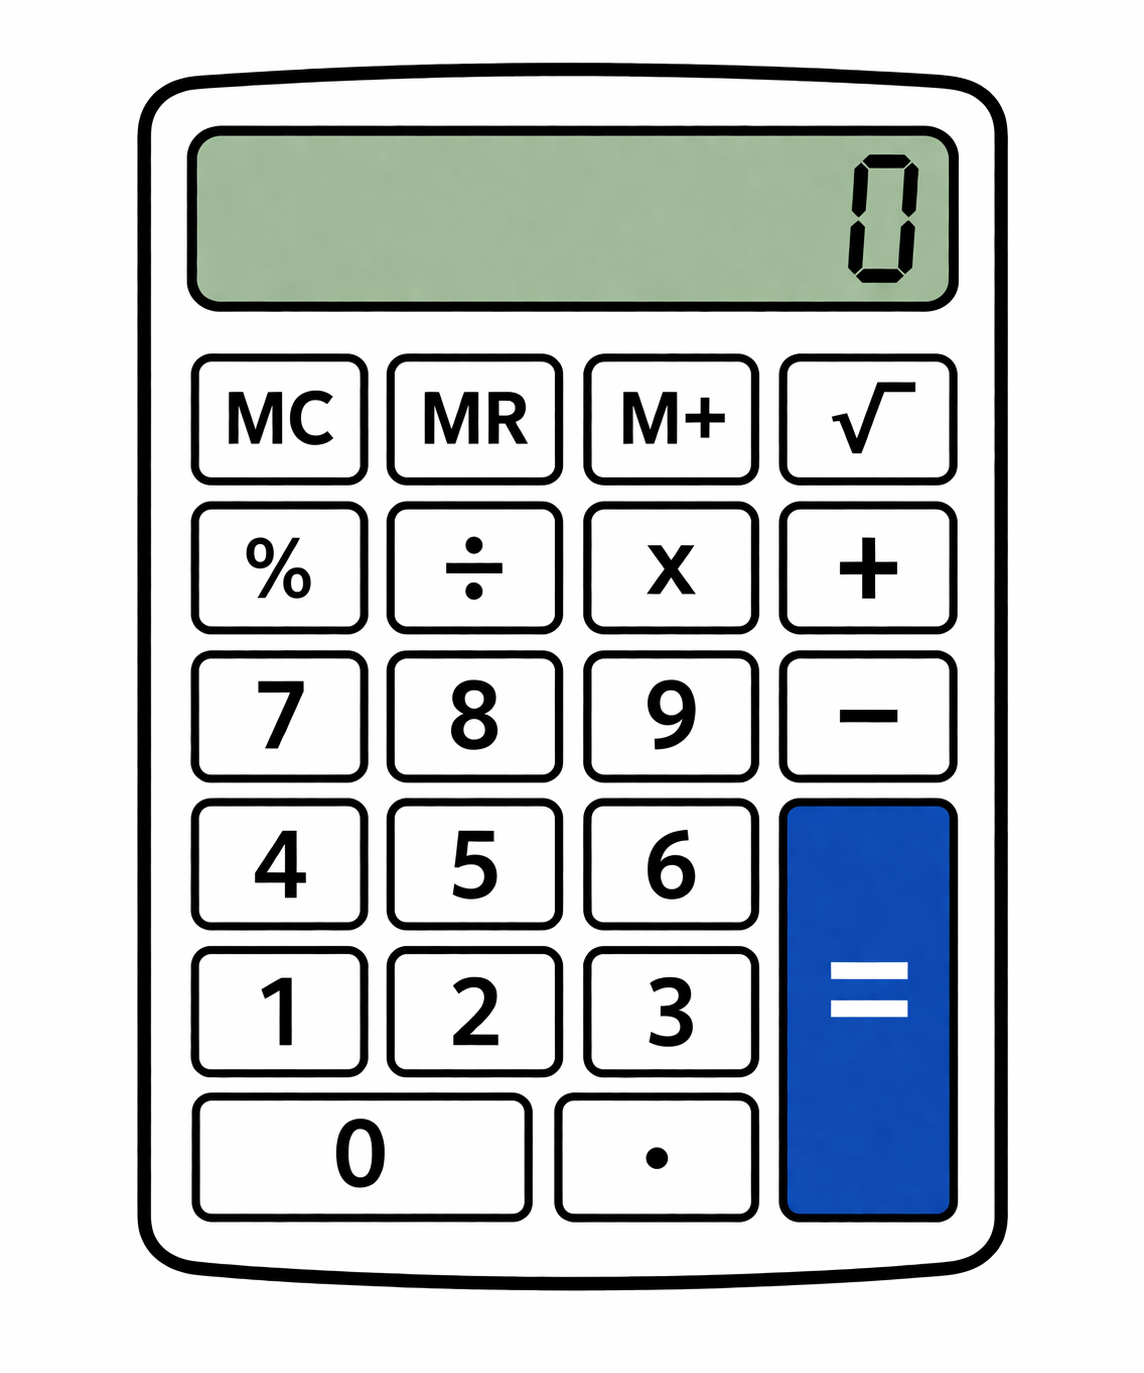
\includegraphics[scale=.15]{calc.png}\end{center}
			\end{framed}

\

	
	\begin{enumerate}
	\itema What is the set of numbers that can be computed exactly in a dollar store calculator \emph{without using} the $\surd$ key?
	\solution{$\Q$}
	
	\
	
	\itema Explain how $\sqrt[4]{2}$ can be computed exactly with a dollar store calculator.
	\solution{$\sqrt{\sqrt{2}}$}
	
	\
	
	\itema Carefully explain\footnote{Hint: Let $\alpha$ be the number that $\surd$ is applied to. Show that the final result must be in $\Q(\sqrt{\alpha})$, and compare $[\Q(\sqrt[n]{2}):\Q]$ with $[\Q(\sqrt{\alpha}):\Q]$.} why neither $\sqrt[3]{2}$ nor $\sqrt[4]{2}$ can be computed exactly with a dollar store calculator using the $\surd$ key \emph{only once} (at any point, not necessarily at the end).
	\solution{Suppose that $\beta$ can be obtained using $\surd$ only once. Let $\alpha\in \Q$ be the number that you apply $\surd$ to. Since any operation after that is essentially $+,-,\times,\div$ with rational numbers, $\beta\in \Q(\sqrt{\alpha})$. Note that $[\Q(\sqrt{\alpha}):\Q]=2$, and $\beta\in \Q(\sqrt{\alpha})$, we must have $[\Q(\sqrt{\alpha}) : \Q] = [\Q(\sqrt{\alpha}) : \Q(\beta)] [\Q(\beta) : \Q]$ by the Degree Formula. Thus $[\Q(\beta) : \Q] \ | \ 2$. However, the minimal polynomial of $\sqrt[3]{2}$ is $x^3-2$ since this is irreducible (by Gauss+Eisenstein) and monic, and has this as a root; thus $[\Q(\sqrt[3]{2}) : \Q] = 3$. This is a contradiction. Similarly for $\sqrt[4]{2}$.}
	
	\
	
	\itema Carefully explain\footnote{Hint: Let $\alpha_1,\alpha_2,\dots,\alpha_n$ be the numbers that $\surd$ is applied to, in order. What can you say about $\Q(\sqrt{\alpha_1},\dots,\sqrt{\alpha_n})$?} why $\pi$  \emph{cannot} be computed exactly with a dollar store calculator. You can use any facts from analysis that we have assumed in this class.
	\solution{Suppose that $\pi$ can be obtained, and let $\alpha_1,\dots,\alpha_n$ be as in the hint. Note that $\Q(\sqrt{\alpha_1},\dots,\sqrt{\alpha_{i+1}})$ is finite, and hence algebraic over $\Q(\sqrt{\alpha_1},\dots,\sqrt{\alpha_{i}})$, since $\sqrt{\alpha_{i+1}}$ is a root of the polynomial $x^2-\alpha_{i+1} \in \Q(\sqrt{\alpha_1},\dots,\sqrt{\alpha_{i}})$ It follows that $\Q(\sqrt{\alpha_1},\dots,\sqrt{\alpha_n})$ is algebraic over $\Q$. Since the final result $\pi$ is in this field, then $\pi$ must be algebraic over $\Q$. This contradicts a fact from analysis.}
	
	\
		\itema Carefully explain\footnotemark[2] why $\sqrt[3]{2}$  \emph{cannot} be computed exactly with a dollar store calculator.
		\solution{Suppose that $\sqrt[3]{2}$ can be obtained, and let $\alpha_1,\dots,\alpha_n$ be as in the hint. The previous argument shows that $[\Q(\sqrt{\alpha_1},\dots,\sqrt{\alpha_{i+1}}) :\Q(\sqrt{\alpha_1},\dots,\sqrt{\alpha_{i}})]$ is at most $2$; in particular, it is either $1$ or $2$ for each $i$. By the Degree Formula, $[\Q(\sqrt{\alpha_1},\dots,\sqrt{\alpha_n}):\Q]=2^k$ for some $k\leq n$. By the argument from (c), we must have $3 \ | \ 2^k$; this is a contradiction.}
			\end{enumerate}
	
\newpage

	\section*{Compass and straightedge constructions}
		\begin{framed}
	A \textbf{classical compass and straightedge construction} is a rule to create from an input finite subset of \emph{marked points}  $S\subseteq \R^2$ another point $Z\in \R^2$ by a sequence of the following rules:
	\begin{itemize}
		\item Take any point $Z\in S$.
	\item If $L$ is the line between two points $P,Q\in S$, and $L'$ is the line between two points $P',Q'\in S$, then adjoin the intersection point $L\cap L'$ to $S$.
	\item If $L$ is the line between two points $P,Q\in S$, and $C$ is the circle centered at $P'\in S$ passing through $Q'\in S$, then adjoin the intersection points $L\cap C$ to $S$.
	\item If $C$ is the circle centered at $P\in S$ passing through $Q\in S$, and $C'$ is the circle centered at $P'\in S$ passing through $Q'\in S$, then adjoin the intersection points $C\cap C'$ to $S$.
	\end{itemize}
	
		\begin{center}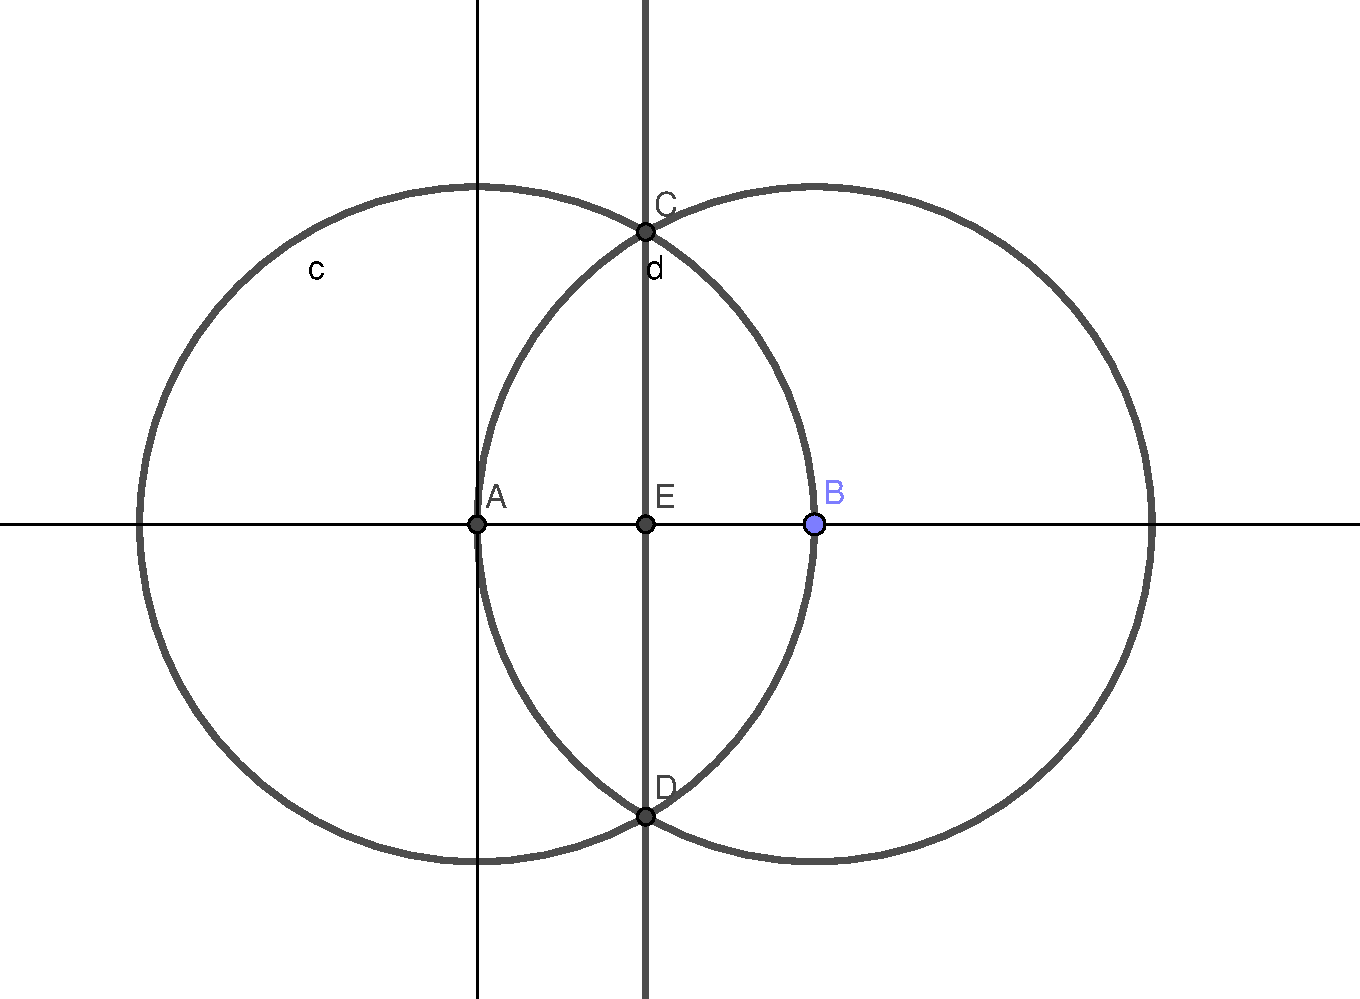
\includegraphics[scale=.3]{constr2.pdf} 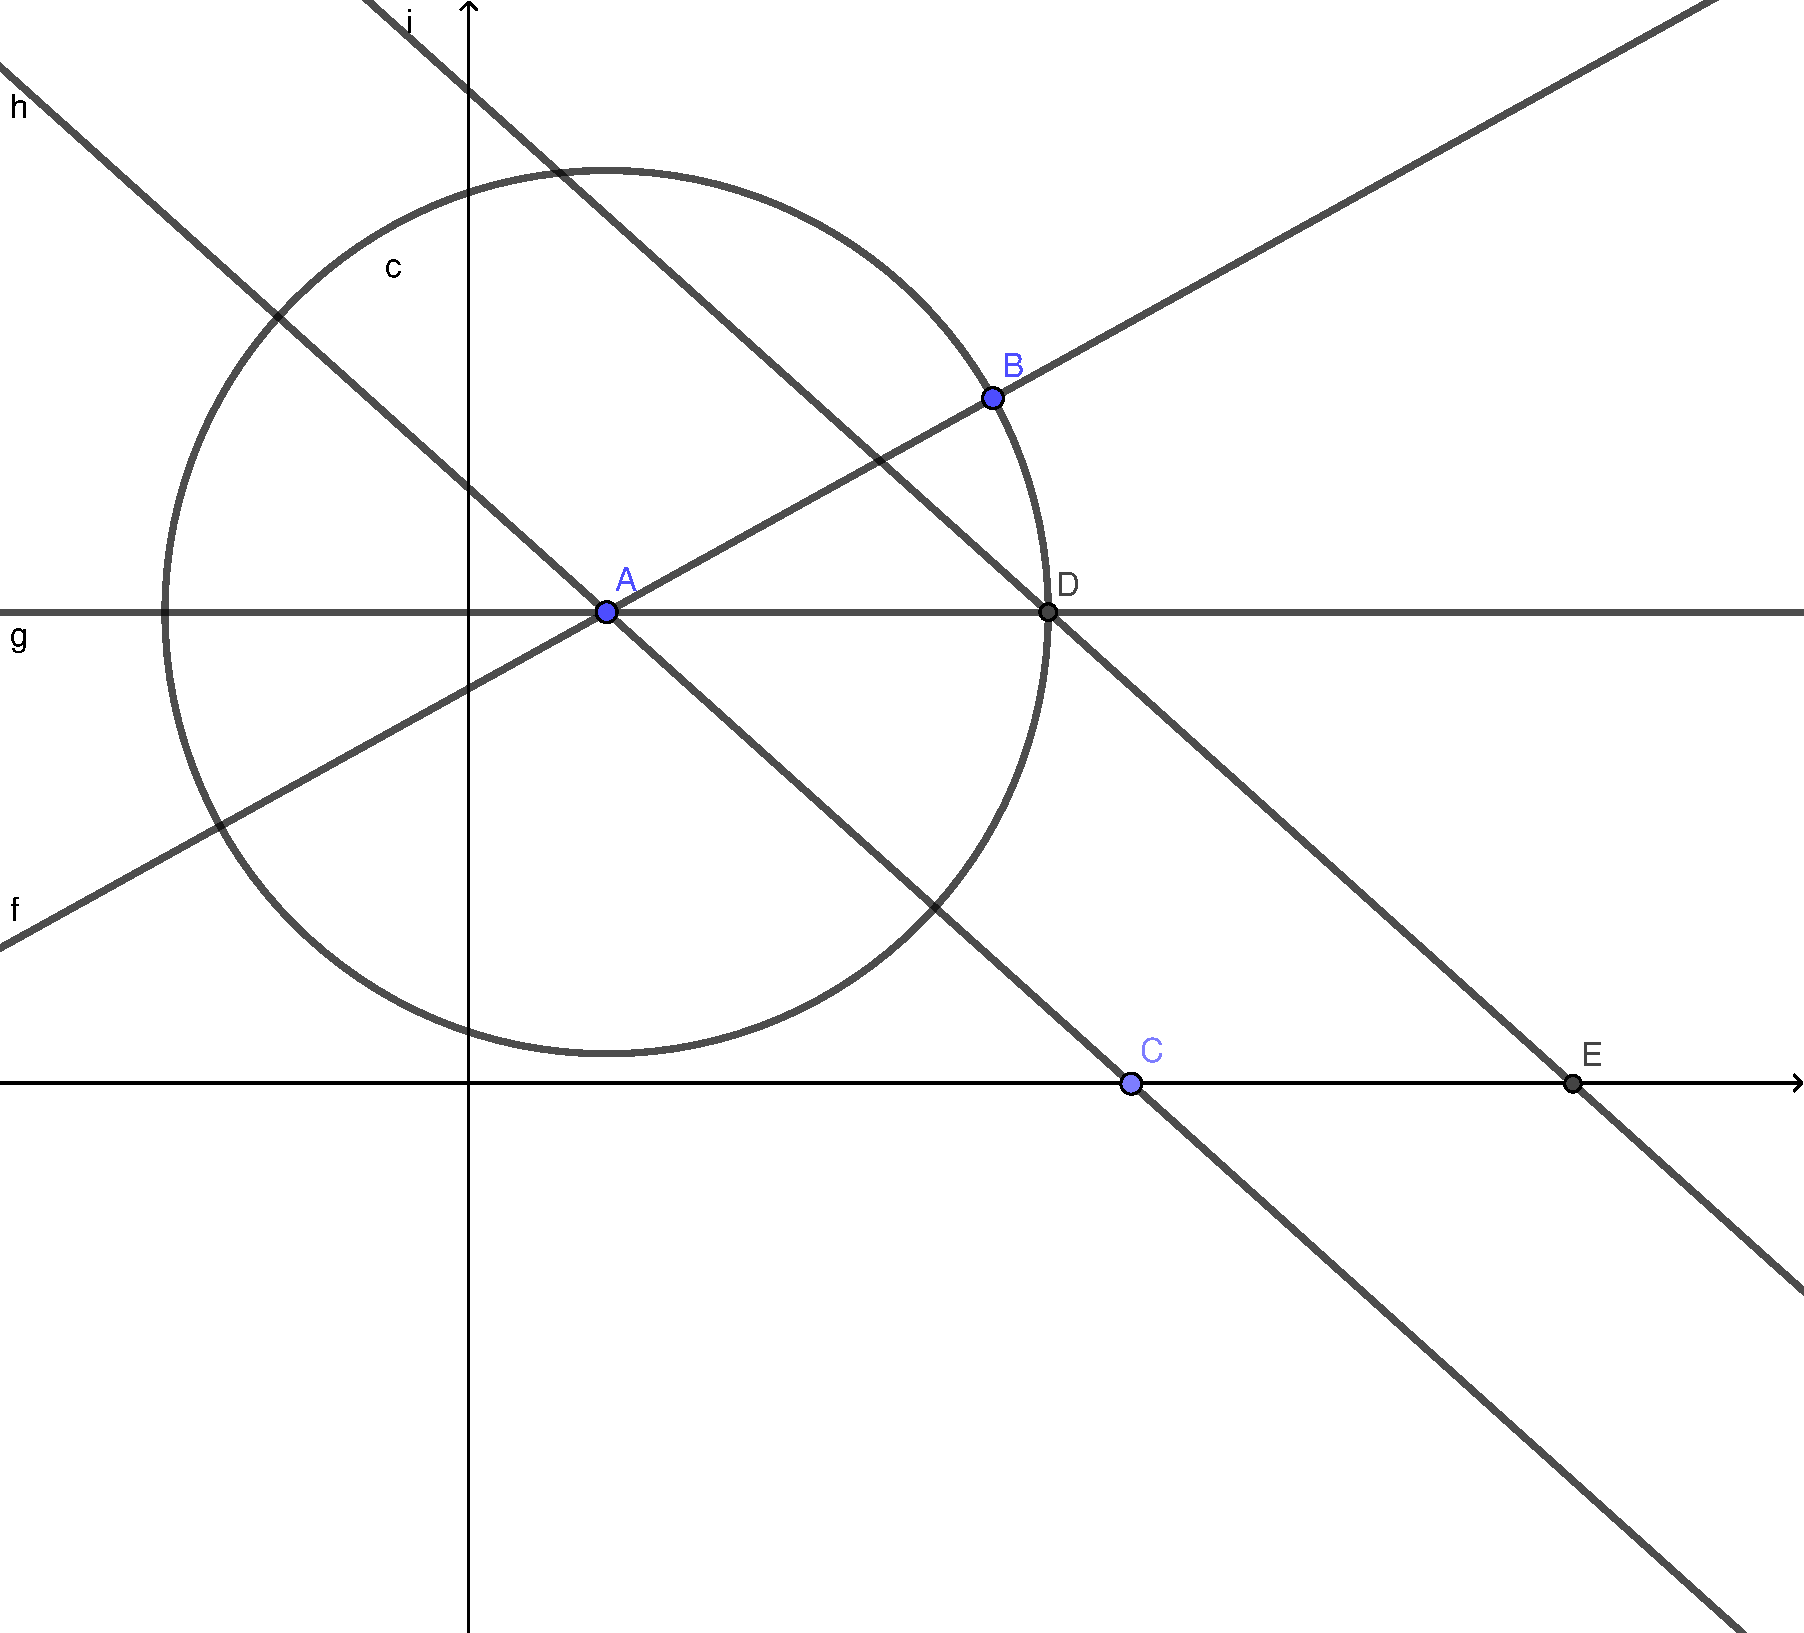
\includegraphics[scale=.2]{cons4.pdf}\end{center}
		
		\
		
\textsc{Lemma:} Given points $P,Q,P',Q'$, the coordinates of a point $X$ in $L\cap L'$, $L\cap C$, or ${C\cap C'}$ as in the constructions above can be computed from the coordinates of $P,Q,P',Q'$ by a sequence of the operations $+,-,\times,\div,\surd$.
	\end{framed} 
	
	\
	
	\begin{enumerate}
	\itemb Suppose that $S=\{(0,0),(1,0)\}$. Use the \textsc{Lemma} to explain why the coordinates of any point that can be obtained from $S$ by a classical compass and straightedge construction can also be obtained from a dollar store calculator.
	
	\
	
	\itemb \textsc{Squaring the circle:} Given two points $P,Q$, show that is impossible to use a classical compass and straightedge construction to give a line segment $\overline{RS}$ such that the area of the square with base $\overline{RS}$ equals the area of the circle with center $P$ passing through $Q$.
	
	\
	
		\itemb \textsc{Doubling the cube:} Given two points $P,Q$, show that is impossible to use a classical compass and straightedge construction to give a line segment $\overline{RS}$ such that the volume of the cube with edge $\overline{RS}$ equals twice the volume of the cube with edge $\overline{PQ}$.	
\end{enumerate}
\end{document}
